\chapter{Working in a simulated environment}

The choice to develop (?) a simulated environment was due to the fact I could not be always in the robotic laboratory, because of other didactic activities. If you do a good job with the abstraction when setting up your simulated robot and world, everything else that was working before, should now continue to work; the goal is to create a simulation as close as possible to the real world, so you can not tell which environment\footnote{real or simulated} you are using.

Part of the setup I am going to present is inspired to Automatic Addison tutorials\cite{tutorials}.

\section{Models}

In order to create a complete simulation, we need to create some models, both for an environment and a robot.

\subsection*{Environment}

It was used a mesh of the Povo upper floors (?), provided by (?). Unfortunately, this is not identical to the real environment, because some measurements are not exact.
The model is written is \Acrfull{sdf} with the mesh as visual and collision model; this model is then used in \code{world} file\footnote{written in \Acrshort{sdf}}, alongside with ground plane and sun ones, provided by Gazebo, and of course the robot model.

\begin{figure}[h]
    \centering
    \includegraphics[width=0.8\textwidth]{images/3d\_povo\_model}
    \caption{Povo model for simulation. Colors are used for a better visualization.}
\end{figure}

\newpage

\subsection*{Robot}

A mesh of robot was created starting from {\it shelfino} (see \autoref{fig:shelfino}), trying to keep it as similar as possible, and each piece\footnote{robot base, lidar, wheels and caster wheel} was exported singularly. For performance reasons, the only mesh actually used is the robot base, because of its special structure, in order to avoid contact with the partially inside spinning wheels. The other ones are substituted by \Acrshort{sdf} or \Acrfull{urdf} built-in geometric shapes.
Both \Acrshort{sdf} and \Acrshort{urdf} are used: the first one is for Gazebo, the second one for a node, called \code{robot\_state\_publisher}, to help visualize the robot (and wheel rotation) in \Acrshort{rviz}.

\begin{figure}[h]
    \centering
    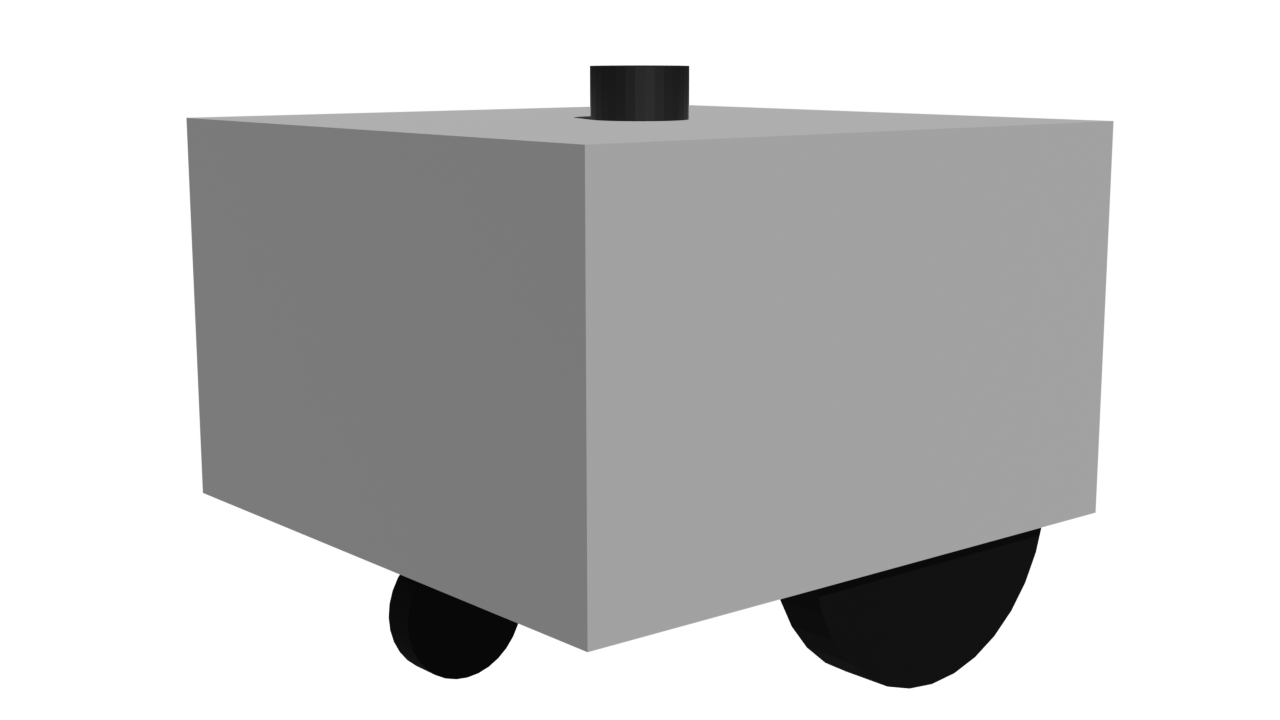
\includegraphics[width=0.7\textwidth]{images/shelfino_3d.png}
    \caption{Shelfino model for simulation.}
\end{figure}

\section{Gazebo plugins}

After placing the models in Gazebo, we need some way to make our robot interact with the environment. It is no longer possible to utilize the nodes in \autoref{subsec:nodes} because they make use of a real hardware, but thankfully, Gazebo provides some plugin that can be attached to the \Acrshort{sdf} model as a normal tag. Once done, robot can be used as if it were a real robot.

\subsection*{Differential drive plugin}

Once added, some configurations needs to be made:
\begin{itemize}
    \item set update rate (Hz)
    \item specify name of wheel joints (control)
    \item wheels separation and diameter (kinematics)
    \item max torque and acceleration (limits)
    \item topics name from where receiving desired velocity and publish odometry data
    \item whether to publish frame transformations and their names (used by \Acrshort{rviz})
\end{itemize}
After that, (the) robot can now move.

\subsection*{Joint state publisher plugin}

This plugin is used to know how much the wheels are spinning in order to visualize the state of the robot in \Acrshort{rviz}. Only update rate and wheel names are required.

\subsection*{Lidar plugin}

When creating a sensor tag of type \code{ray}, with scan (direction, angle, number of samples), range (distance) and noise (disturbance) information, a lidar plugin should be added. Only configurations needed are:
\begin{itemize}
    \item topic name where to pub the data
    \item which \Acrshort{ros} message type to use (sensor\_msgs/LaserScan)
    \item frame name where the lidar is attacched to
\end{itemize}

% add robot description of link, joints, ecc...? o qualcos'altro? tipo sdf come allegato? (?)